\usetikzlibrary{calc,angles,quotes}
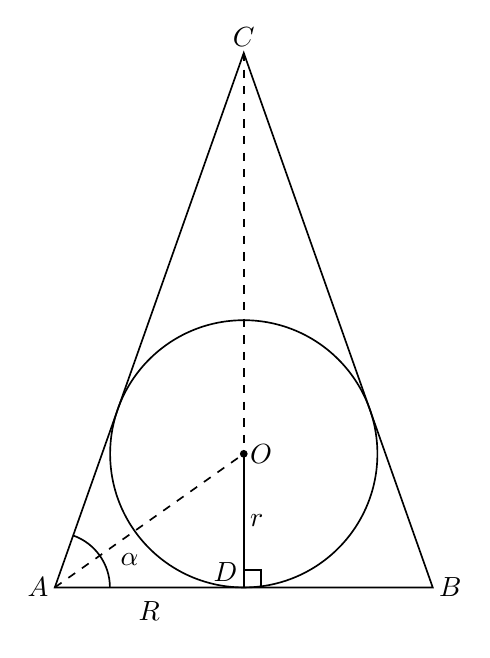
\begin{tikzpicture}[x=1cm,y=1cm,line width=.6pt,font=\normalsize]
\coordinate (A) at (-2.4,0.0);
\coordinate (B) at (2.4,0.0);
\coordinate (D) at (0.0,0.0);
\coordinate (C) at (0.0,6.7882);
\coordinate (O) at (0.0,1.6971);
\draw (C)--(A)--(B)--cycle;
\draw[dashed] (C)--(D);
\draw[dashed] (A)--(O);
\draw (O)--(D);
\draw (O) circle[radius=1.6971cm];
\draw (0,0.22)--(0.22,0.22)--(0.22,0);
\draw (A)+(0.7,0) arc[start angle=0,end angle=70.53,radius=0.7cm];
\node[left=2pt,inner sep=0pt] at (A) {$A$};
\node[right=2pt,inner sep=0pt] at (B) {$B$};
\node[above=2pt,inner sep=0pt] at (C) {$C$};
\node[above left=2pt,inner sep=0pt] at (D) {$D$};
\node[right=2pt,inner sep=0pt] at (O) {$O$};
\node[right=2pt,inner sep=0pt] at (0,0.85) {$r$};
\node[below] at (-1.2,-0.05) {$R$};
\node at (-1.45,0.35) {$\alpha$};

% Explicit named circle-center points, painted after all region fills.
\fill (O) circle[radius=1.4pt];
\end{tikzpicture}
